%###########################PRESENTACION##########################################
%Modo presentación
\documentclass[12pt]{beamer}

%Modo handout
%\documentclass[handout,compress]{beamer}
%\usepackage{pgfpages}
%\pgfpagesuselayout{4 on 1}[border shrink=1mm]

\usepackage{graphicx}
\usepackage{beamerthemeCambridgeUS}
\usepackage{ragged2e}
\usepackage{multimedia}
\usepackage{subfig}
\usepackage{tikz}
\usepackage{amsmath}
\setbeamercovered{transparent}
\usepackage{textpos} 


\graphicspath{{G:/My Drive/FIGURAS/}}

\title[Introducción]{ANÁLISIS GEOESPACIAL}
\author[Edier Aristizábal]{Edier V. Aristizábal G.}
\institute{\emph{evaristizabalg@unal.edu.co}}
\date{(Versión:\today)}


\addtobeamertemplate{headline}{}{%
	\begin{textblock*}{2mm}(.9\textwidth,0cm)
	\hfill
\includegraphics[height=1cm]{un.png}  
	\end{textblock*}
			}
%############################INICIO#############################################
\begin{document}
%###########################SLIDE
\begin{frame}
\titlepage
\centering
	
\includegraphics[width=5cm]{unal.png}\hspace*{4.75cm}~%
   	
\includegraphics[width=2cm]{logo3} 
\end{frame}
%#############################SLIDE
\begin{frame}
\centering
	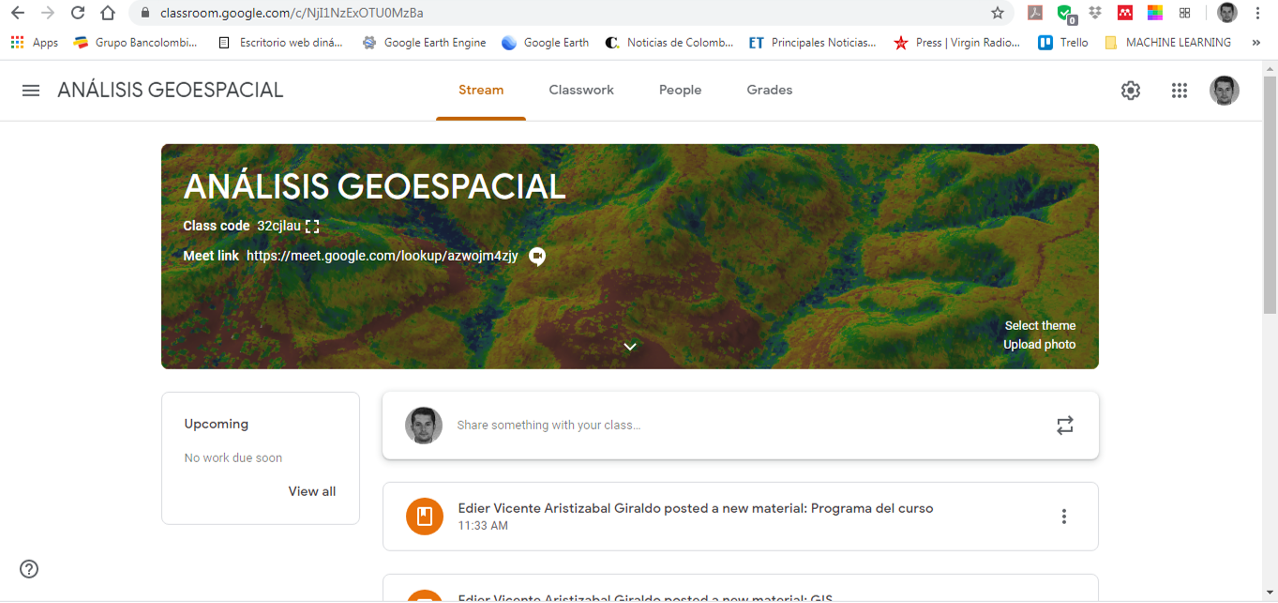
\includegraphics[width=12cm]{curso}
\end{frame}
%#############################SLIDE
 \begin{frame}
\centering
	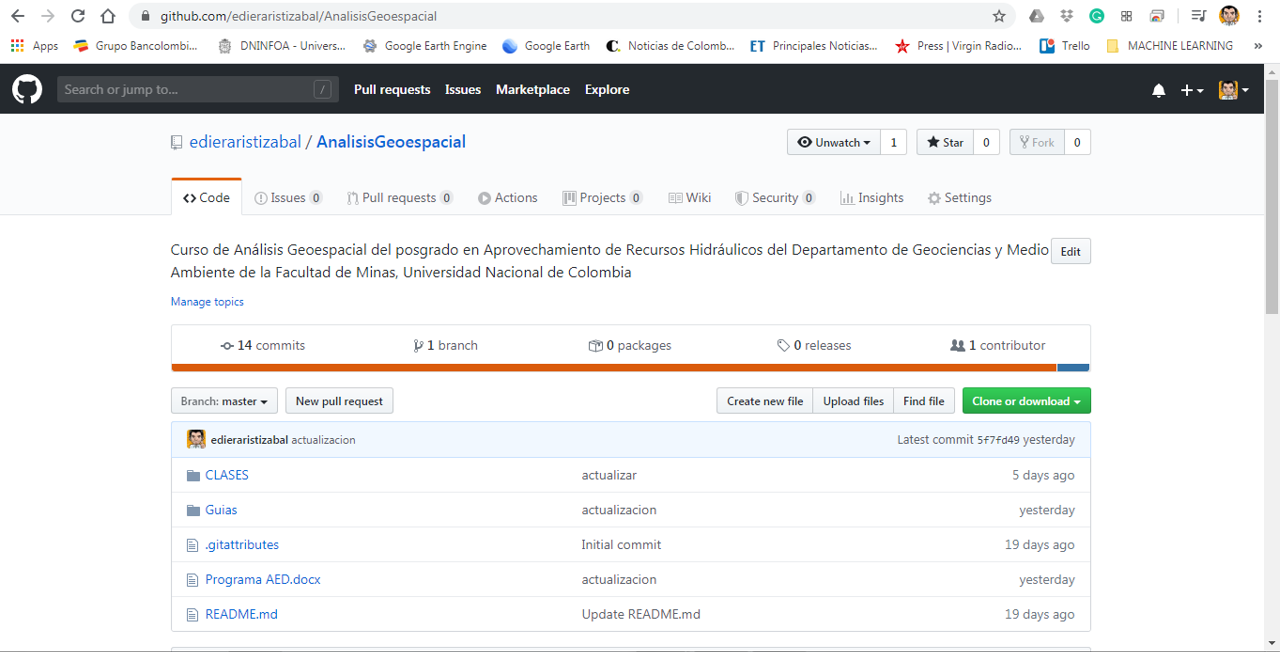
\includegraphics[width=12cm]{github}
\end{frame}
 %#############################SLIDE
\begin{frame}
\frametitle{Objetivos del curso}
\framesubtitle{Objetivos y alcances del curso}
\justifying
El curso \alert{Análisis Geoespacial} está orientado para estudiantes de posgrados que deseen formarse como GDS (Geospatial Data Science) adquiriendo conocimientos sobre sensores remotos y datos geoespaciales en un contexto ambiental, utilizando herramientas tipo Sistemas de Información Geográfica (SIG), Google Earth Engine (GEE), QGIS, Big Data, y programación en lenguaje Python.\vfill

El curso es teórico - práctico. Se dictarán clases teóricas con las técnicas y modelos a utilizar, y clases prácticas donde se resolverán dudas con el manejo de las herramientas. El curso se evaluará a través de un trabajo individual durante todo el curso, donde el estudiante implementará en una cuenca de su elección las herramientas de análisis presentadas en el curso.
\end{frame}
 %#############################SLIDE
\begin{frame}
\begin{block}{\emph{Geospatial Data Science}}
\justifying
\small{Geospatial data science (GDS) is a subset of Data Science that focuses on the unique characteristics of spatial data, moving beyond simply looking at \textbf{where things happen to understand why they happen there}}.
\end{block}
\centering
	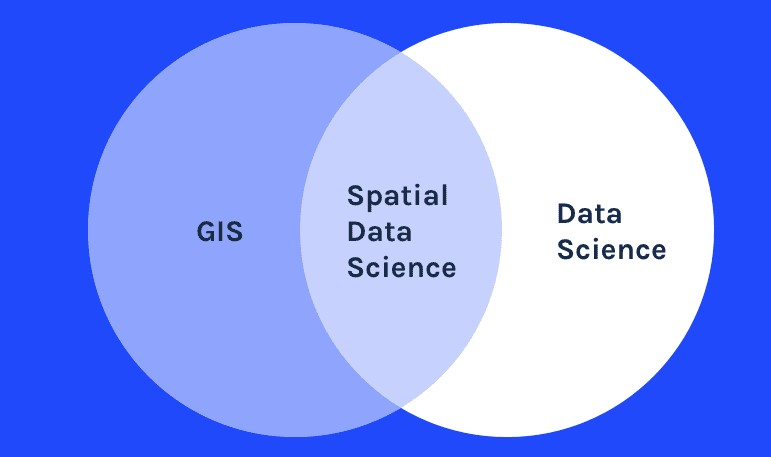
\includegraphics[width=4.5cm]{sds}\vfill
\tiny{https://carto.com/what-is-spatial-data-science/}
\end{frame}
 %#############################SLIDE
\begin{frame}
\frametitle{\emph{Geospatial Data Science}}
\centering
	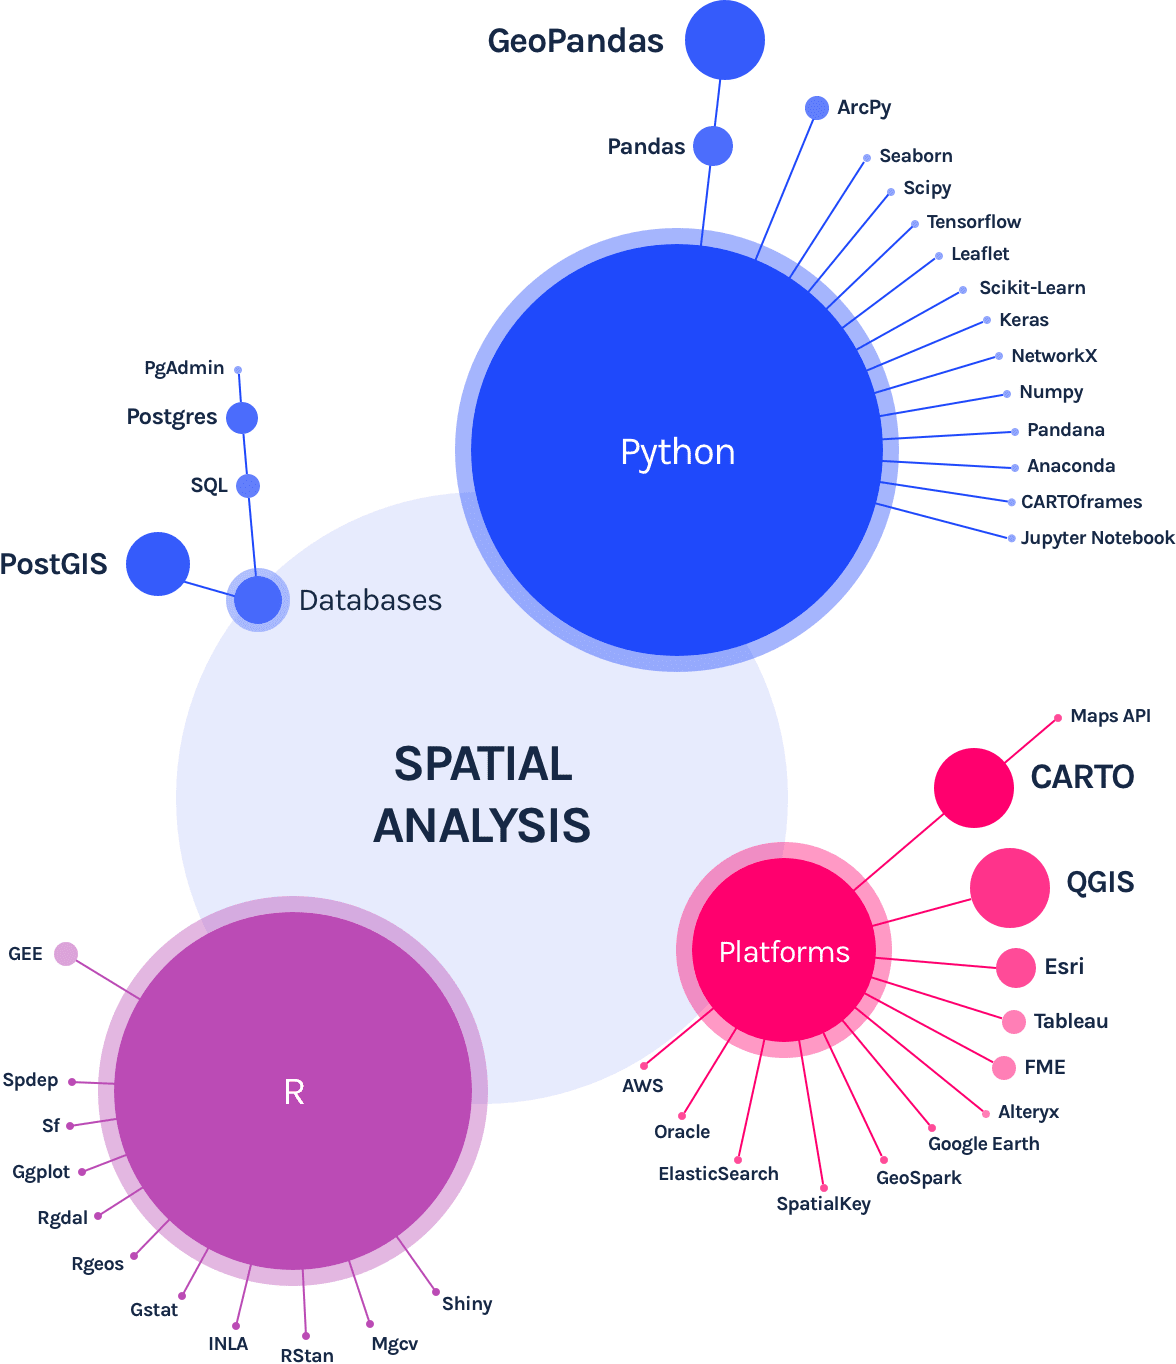
\includegraphics[width=6cm]{spatialdatascience}\vfill
	\tiny{https://carto.com/what-is-spatial-data-science/}
\end{frame}
 %#############################SLIDE
\begin{frame}
\centering
	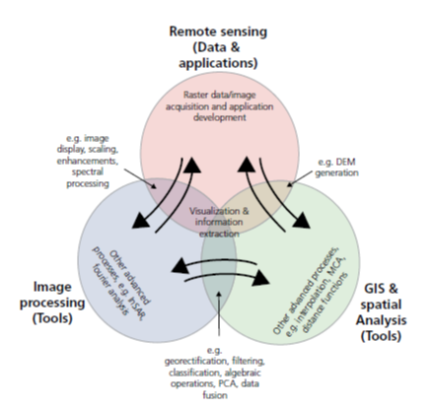
\includegraphics[width=8cm]{ven}
\end{frame}
 %#############################SLIDE
 \begin{frame}
\frametitle{\emph{Why spatial is special?}}
\centering
	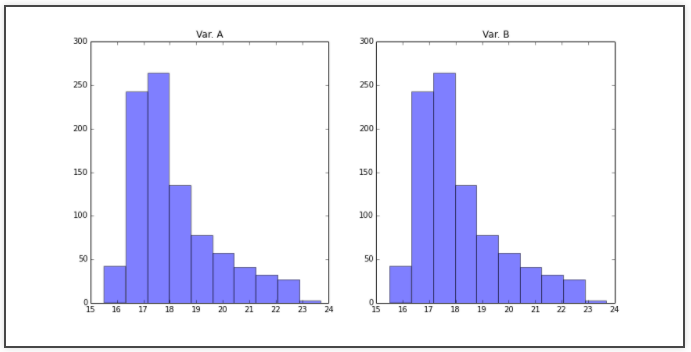
\includegraphics[width=11cm]{london}
\end{frame}
 %#############################SLIDE
  \begin{frame}
\frametitle{\emph{Why spatial is special?}}
\centering
	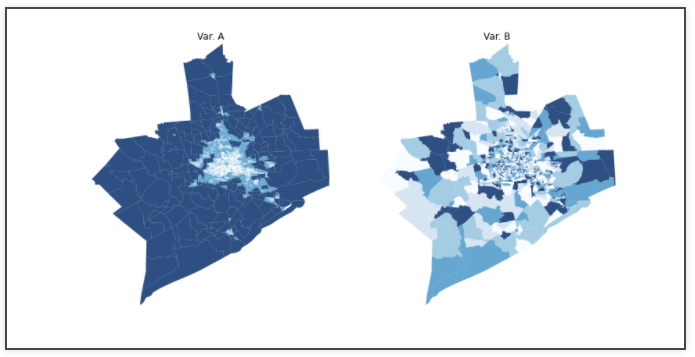
\includegraphics[width=11cm]{london1}
\end{frame}
 %#############################SLIDE
\begin{frame}
\centering
	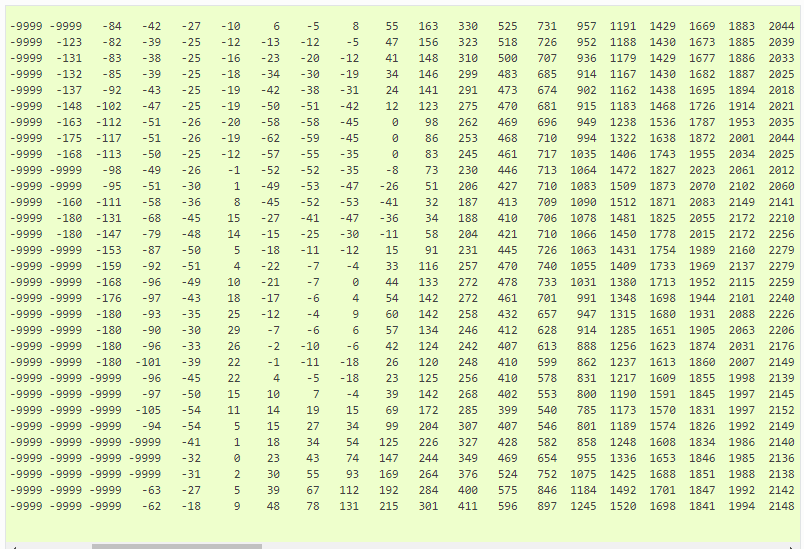
\includegraphics[width=10cm]{temp}\vfill
\tiny{https://geo-python.github.io/site/lessons/L1/motivation.html}
\end{frame}
 %#############################SLIDE
\begin{frame}
\centering
	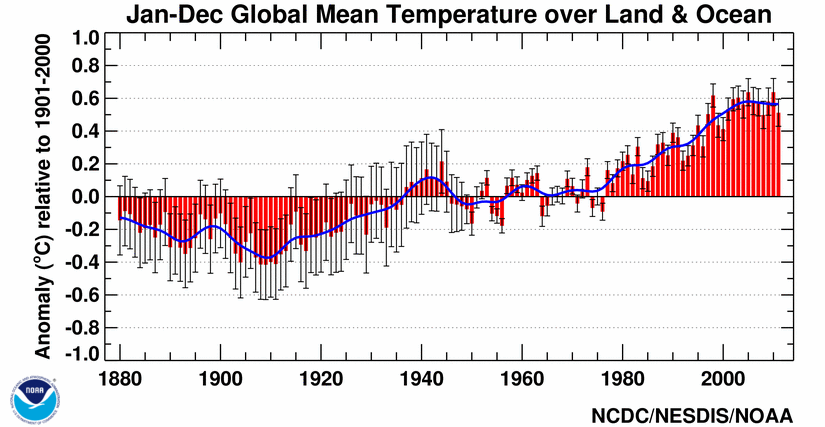
\includegraphics[width=10cm]{temp2}\vfill
\tiny{Global mean temperature anomalies from 1880-2011. Source: https://www.ncdc.noaa.gov/sotc/global/201113}
\end{frame}
 %#############################SLIDE
\begin{frame}
\centering
	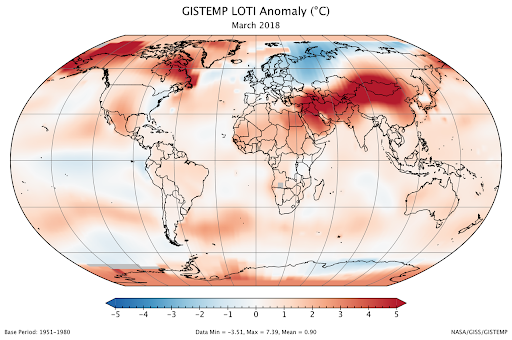
\includegraphics[width=10cm]{temp3}\vfill
\tiny{Global temperature anomalies for March 2018. Source: https://www.ncdc.noaa.gov/sotc/global/201803}
\end{frame}
%#############################SLIDE
\begin{frame}
\centering
	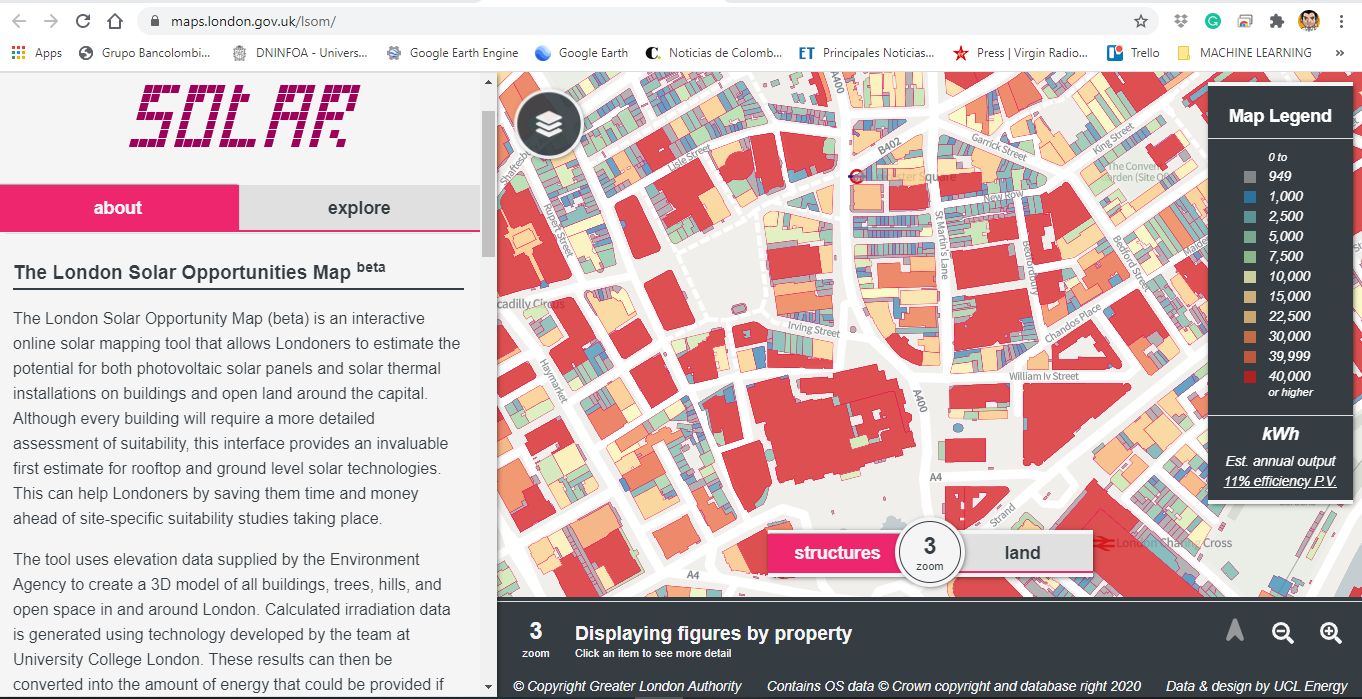
\includegraphics[width=12cm]{solar-london}
\url{https://maps.london.gov.uk/lsom/}
\end{frame}
%#############################SLIDE
\begin{frame}
\centering
	\includegraphics[width=12cm]{progra}
\end{frame}
%#############################SLIDE
\begin{frame}
\centering
	\includegraphics[width=12cm]{program2}
\end{frame}
%#############################SLIDE
\begin{frame}
\centering
	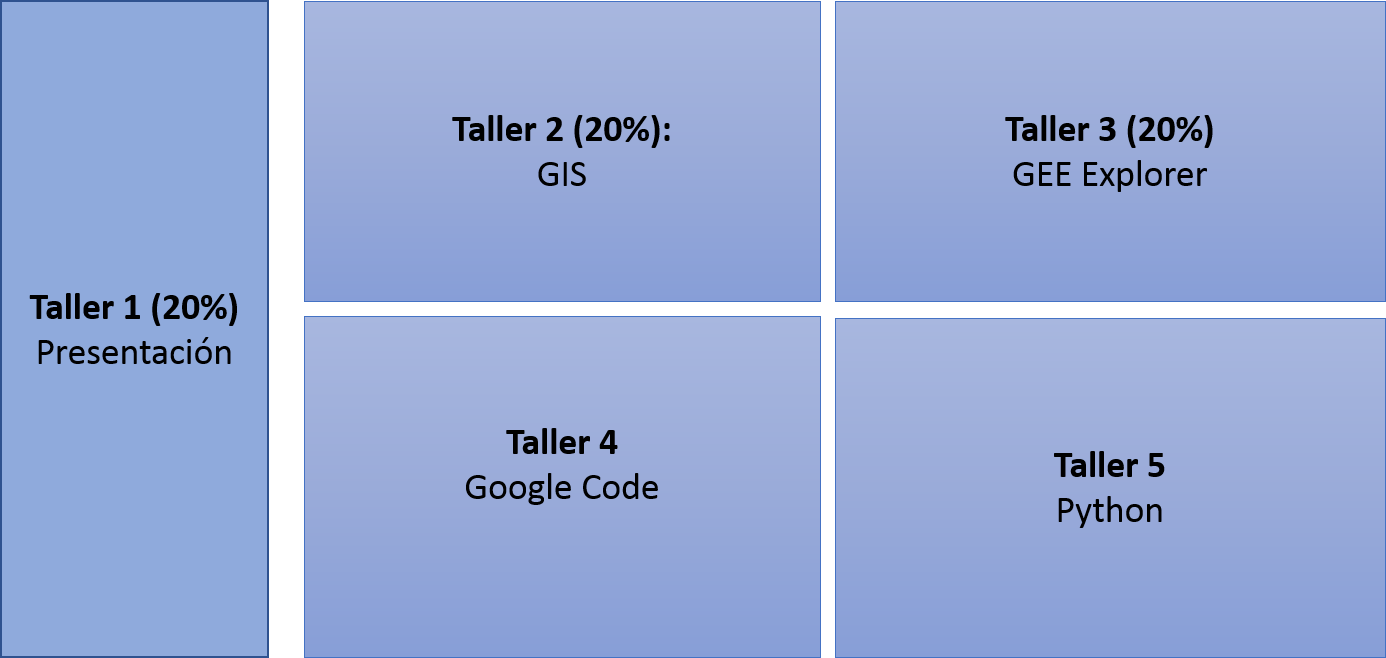
\includegraphics[width=12cm]{eval}
\end{frame}
%#############################SLIDE
\end{document}